\documentclass{tufte-handout}
\usepackage{amsmath}
\usepackage{mathpazo}

\usepackage{tikz}
\usetikzlibrary{chains}
% Define style for nodes
\tikzstyle{every node}=[circle, draw, fill=white,
                        inner sep=0pt, minimum width=9pt,font=\footnotesize\sf]
\tikzstyle{every picture}= [scale=.5,baseline=(current bounding box.center)]
\usetikzlibrary{automata}
\usetikzlibrary{patterns}
\usepackage{booktabs}
\usepackage{siunitx}
\IfFileExists{vc.tex}{\input{vc.tex}}{\newcommand\GITAuthorDate{no git info found}\newcommand\GITAbrHash{-}}  % For version control

\title{Heaps}
\author{}
\date{\GITAuthorDate, rev. \GITAbrHash}

\begin{document}
\maketitle
%\section{}
%\subsection{}

\begin{abstract}
  This is about heaps
\end{abstract}

\section{\textbf{Question 1}: 150819 3a}
Insert the keys {\tt 1 3 6 2 4 5} in that order into a heap. Draw the result.

\section{\textbf{Question 2}: 170815 3a, e, f}
\begin{description}
  \item[(3a)] 
    Consider a Stack $S$, implementated as a linked list.
    Beginning with an empty data structure, assume I called
    {\tt S.push("World");} 
    {\tt S.push("World");} 
    {\tt S.pop();}, and 
    {\tt S.push("Hello");}.
    How does the data structure look after these operations?

    (a)
    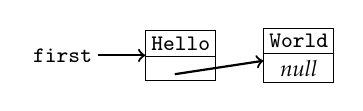
\begin{tikzpicture}
      \node[draw = none,rectangle,inner sep = 2pt] (first) at (-3,0) {{\tt first}};
      \node[rectangle split, rectangle split parts = 2, inner sep = 2pt]
	(hello) { {\tt Hello} \nodepart{second} };
      \node[rectangle split, rectangle split parts = 2, inner sep = 2pt]
	(world) at (3,0)
	{ {\tt World} \nodepart{second} {\rm\em null}};
	\draw[->, thick] (first)--(hello);
	\draw[->, thick] (hello.second)--(world);
      \end{tikzpicture}

     (b)
    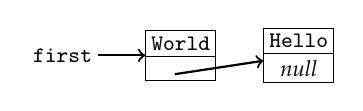
\begin{tikzpicture}
      \node[draw = none,rectangle,inner sep = 2pt] (first) at (-3,0) {{\tt first}};
      \node[rectangle split, rectangle split parts = 2, inner sep = 2pt]
	(world) { {\tt World} \nodepart{second} };
      \node[rectangle split, rectangle split parts = 2, inner sep = 2pt]
	(hello) at (3,0)
	{ {\tt Hello} \nodepart{second} {\rm\em null}};
	\draw[->, thick] (first)--(world);
	\draw[->, thick] (world.second)--(hello);
    \end{tikzpicture}

    (c)
    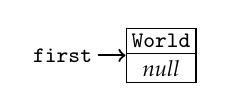
\begin{tikzpicture}
      \node[draw = none,rectangle,inner sep = 2pt] (first) at (.5,0) {{\tt first}};
      \node[rectangle split, rectangle split parts = 2, inner sep = 2pt]
	(world) at (3,0)
	{ {\tt World} \nodepart{second} {\rm\em null}};
	\draw[->, thick] (first)--(world);
    \end{tikzpicture}

    (d)
    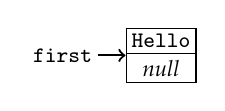
\begin{tikzpicture}
      \node[draw = none,rectangle,inner sep = 2pt] (first) at (.5,0) {{\tt first}};
      \node[rectangle split, rectangle split parts = 2, inner sep = 2pt]
	(hello) at (3,0)
	{ {\tt Hello} \nodepart{second} {\rm\em null}};
	\draw[->, thick] (first)--(hello);
    \end{tikzpicture}


  \medskip\item[(3e)]
  Consider a quick-find implementation of Union--Find with 5 elements.
  After some operations, the internal data structure looks like this:

  \begin{tabular}{ccccc}
    \multicolumn{5}{c}{\tt id[]}\\
  0 & 1 & 2 & 3 & 4 \\ 	\hline
  0 & 1 & 2 & 2 & 4 
  \end{tabular}

  Assume we now union elements 2 and 4. How does the resulting data structure look?

  \medskip\item[(3f)]
    In which sense is it Quick-union better than Quick-find? 
      \begin{enumerate}
        \item The union operation is asymptotically faster. 
        \item The amortized complexity of find is asymptotically faster. 
        \item It can compute a minimum forest. 
        \item It uses less space.
      \end{enumerate}
\end{description}

\section{\textbf{Question 3}: [SW] 2.4.27 }


\section{\textbf{Question 4}: [SW] 2.4.30 }

\end{document}